% 24th, Jan, 2001 Ver.1     Tatsuya Okabe
%                 Ver.2
%                 Ver.3
%                 Ver.4
%                 Ver.5
%
%---------------------------------------------------------------------------%
% Made by Tatsuya Okabe ( HONDA R&D Europe ( Deutschland ) GmbH )           %
% Checked by Bernhard Sendhoff ( HONDA R&D Europe ( Deutschland ) GmbH )    %
%---------------------------------------------------------------------------%
% Class Weibull

\section{Abstract}

\noindent
With the class {\em Weibull}, we can simulate the ``Weibull''
distribution. This distribution follows the equation :

\begin{equation}
f(x) = \frac{\alpha}{\beta} \cdot \exp \left\{ - \frac{1}{\beta} x^\alpha \right\} \cdot x^{\alpha-1}
\end{equation}

\noindent
In this equation, $\alpha$, $\beta$ and x mean the constant variable, the constant
variable and the factor, respectively.

\vspace*{10mm}

\begin{center}
\begin{figure}[h]
\rotatebox{-90}{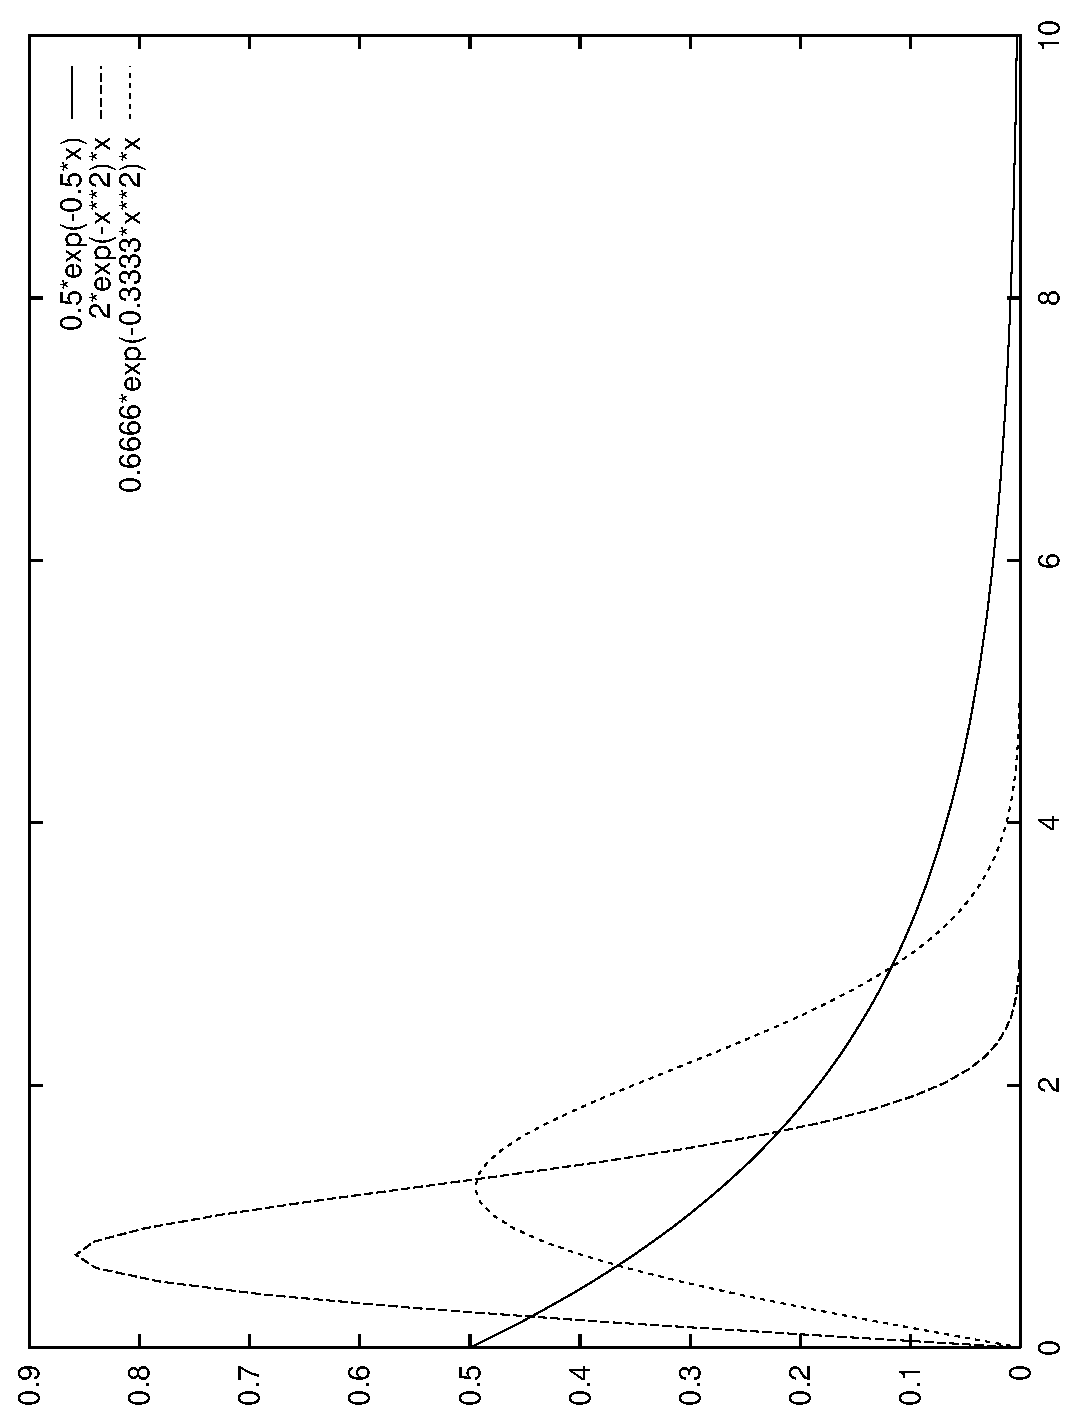
\includegraphics[height=12cm]{weibull.eps}}\\
\caption{The Weibull distribution $(\alpha ,\beta
)=(1,2),(2,1),(2,3)$.}
\end{figure}
\end{center}

\clearpage

\section{Internal Variables}

\begin{itemize}
\item pAlpha - The constant variable $\alpha$.
\item pBeta - The constant variable $\beta$.
\end{itemize}

%********************
\index{pAlpha (Variable)}
\index{pBeta (Variable)}
%********************

\vspace*{10mm}

\section{Public Methods}

\noindent
These methods can be used by all \cpp - programs, that have included the
header file Weibull.h and the library EA. If you declare only
Population.h, we can't use these methods in this version.

\subsection{Constructors}

%---------------------------------------------------------------------------%
% 001
\index{Weibull!( double alpha, double beta )}
\setNormalInstance
\setCorrectWidthThree{8pt}
\setParamOne{alpha}{double}{The constant variable $\alpha$.} 
\setParamTwo{beta}{double}{The constant variable $\beta$.}
\printMethodWithParamsSaved
{}
{None.}
{Weibull}
{The default constructor. Generates the random generator of Weibull distribution.}
{None.}
\setCorrectWidthThree{4pt}
%---------------------------------------------------------------------------%

%---------------------------------------------------------------------------%
% 002
\index{Weibull!( double alpha, double beta, RNG\& rng )}
\setNormalInstance
\setCorrectWidthThree{8pt}
\setParamOne{alpha}{double}{The constant variable $\alpha$.} 
\setParamTwo{beta}{double}{The constant variable $\beta$.}
\setParamThree{rng}{RNG\&}{RNG class.}
\printMethodWithParamsSaved
{}
{None.}
{Weibull}
{The constructor. Generates the random generator of Weibull distribution.}
{None.}
\setCorrectWidthThree{4pt}
%---------------------------------------------------------------------------%

\clearpage

\subsection{Operators}

%---------------------------------------------------------------------------%
% 003
\index{operator( )!( double alpha, double beta )}
\setNormalInstance
\setCorrectWidthThree{8pt}
\setParamOne{alpha}{double}{The constant variable $\alpha$.} 
\setParamTwo{beta}{double}{The constant variable $\beta$.}
\printMethodWithParamsSaved
{double}
{The result of Weibull distribution.}
{operator( )}
{Gets the result of Weibull distribution.}
{None.}
\setCorrectWidthThree{4pt}
%---------------------------------------------------------------------------%

%---------------------------------------------------------------------------%
% 004
\index{operator( )!( )} 
\setNormalInstance
\printEmptyMethodReturnSpecial
{double}
{operator( )}
{Gets the result of Weibull distribution.}
{The result of Weibull distribution.}
{None.}
%---------------------------------------------------------------------------%

\vspace*{10mm}

\subsection{Information Retrieval Methods}

%---------------------------------------------------------------------------%
% 005
\index{alpha!( )} 
\setConstInstance
\printEmptyMethodReturnSpecial
{double}
{alpha}
{Returns the constant variable {\em pAlpha}.}
{The constant variable {\em pAlpha}.}
{None.}
%---------------------------------------------------------------------------%

%---------------------------------------------------------------------------%
% 006
\index{beta!( )} 
\setConstInstance
\printEmptyMethodReturnSpecial
{double}
{beta}
{Returns the constant variable {\em pBeta}.}
{The constant variable {\em pBeta}.}
{None.}
%---------------------------------------------------------------------------%

\clearpage

%---------------------------------------------------------------------------%
% 007
\index{alpha!( double a )} 
\setNormalInstance
\printMethodWithOneParam
{void}
{aplha}
{double}
{a}
{New value of the constant variable {\em pAlpha}.}
{Sets the variable {\em pAlpha} using new variable {\em a}.}
{None.}
{None.}
%---------------------------------------------------------------------------%

%---------------------------------------------------------------------------%
% 008
\index{beta!( double b )} 
\setNormalInstance
\printMethodWithOneParam
{void}
{beta}
{double}
{b}
{New value of the constant variable {\em pBeta}.}
{Sets the variable {\em pBeta} using new variable {\em b}.}
{None.}
{None.}
%---------------------------------------------------------------------------%

\vspace*{10mm}

\subsection{The probability}

%---------------------------------------------------------------------------%
% 010
\index{p!( const double\& x )} 
\setConstInstance
\printMethodWithOneParam
{double}
{p}
{const double\&}
{x}
{The factor which you want to calculate the probability.}
{Returns the probability of {\em x}.}
{The probability.}
{None.}
%---------------------------------------------------------------------------%













